% $HeadURL$

\paragraph{Simple chemical}
\label{sec:simpleChemical}

A simple chemical in SBGN is defined as the opposite of a
macromolecule (\sect{macromolecule}): it is a chemical compound that
is \emph{not} formed by the covalent linking of pseudo-identical
residues.  Examples of simple chemicals are an atom, a monoatomic ion,
a salt, a radical, a solid metal, a crystal, etc. The complex can be
represented by a monomeric glyph (\glyph{Simple chemical monomer}) and a multimeric
glyph (\glyph{Simple chemical multimer}).


\begin{glyphDescription}
% \item[Identifying Attributes:]\mbox{}
%   \begin{itemize}
%   \item owning compartment
%   \item name
%   \item cardinality
%   \end{itemize}
\begin{glyphIdentity}
  \item owning compartment
  \item name
  \item cardinality
\end{glyphIdentity}
\glyphRules The mutimer glyph
  must be used if cardinality is greater than 1.
\end{glyphDescription}


\subparagraph{Glyph: \glyph{Simple chemical monomer}}

This glyph is used to represent a simple chemical with a cardinality
of one.

\begin{glyphDescription}

\glyphSboTerm SBO:0000247 ! simple chemical

\glyphContainer A \glyph{simple chemical} is represented by a circular
container, as depicted in \fig{simpleChemical}. To avoid confusion
with the Unspecified Entity (\ref{sec:unspecifiedEntity}), this glyph
must remain a circle and cannot be deformed into an eclipse.

\glyphLabel The identification of the \glyph{simple chemical} is carried by an unbordered box containing a string of characters.  The characters may be distributed on several lines to improve readability, although this is not mandatory.  The label box has to be attached to the center of the circular container.  The label is permitted to spill outside the container.

\glyphAux A \glyph{simple chemical} may be decorated with one or more \glyph{units of information} (\sect{unitInfo}).  A particular \glyph{unit of information} describes the material type.  A \glyph{simple chemical} may also carry a \glyph{clone marker} (\sect{cloneMarker}).

\glyphCloning Simple Clone Marker

\end{glyphDescription}

\begin{figure}[H]
  \centering
  
\includegraphics[scale = 0.3]{images/simpleChemical}
  \caption{The \PD glyph for \glyph{simple chemical}.}
  \label{fig:simpleChemical}
\end{figure}

\subparagraph{Glyph: \glyph{Simple chemical multimer}}

This glyph is used to represent a simple chemical with a cardinality
of one.

\begin{glyphDescription}

\glyphSboTerm SBO:0000421 ! multimer of simple chemicals

\glyphContainer A \glyph{simple chemical multimer} is represented by two identical containers shifted horizontally and vertically and stacked one on top of the other.  \fig{multimer} illustrates the glyph.

\glyphLabel A \glyph{multimer} has no identity on its own.  However, the first of the monomers carries an identifying label.  The label is placed in an unbordered box containing a string of characters.  The characters can be distributed on several lines to improve readability, although this is not mandatory.  The label box must be attached to the center of the top monomer's container.  The label may spill outside of the container.

\glyphAux A \glyph{multimer} can carry state variables that can add information about its state (\sect{stateVariable}).  The state of a multimer is therefore defined as the vector of all its state variables.  Note that a \glyph{state variable} carried by a multimer actually applies to each of the constituent monomers individually.  If instead the state variables are meant to apply to the whole multimeric assembly, a \glyph{macromolecule} (\sect{macromolecule}) should be used instead of \glyph{multimer}.  An assembly containing some state variables applicable to the components, and others state variable applicable to the assembly (for instance opening of a channel and phosphorylation of each of its subunits) should be represented by a \glyph{complex} (\sect{complex}).

\glyphCloning Simple Clone Marker

\end{glyphDescription}

\begin{figure}[H]
  \centering
  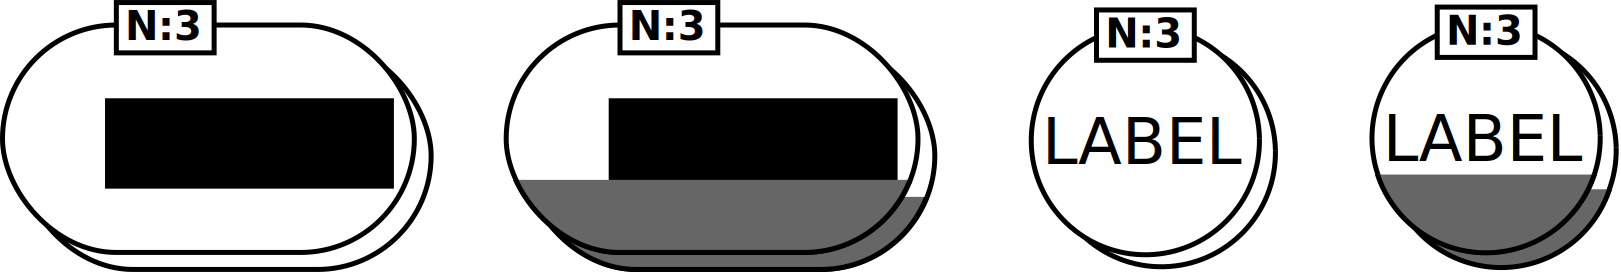
\includegraphics[scale = 0.3]{images/simpleChemicalMultimer}
  \caption{The \PD glyph for \glyph{multimer}.}
  \label{fig:multimer}
\end{figure}

% The following is for [X]Emacs users.  Please leave in place.
% Local Variables:
% TeX-master: "../sbgn_PD-level1"
% End:

